% OVERVIEW
\subsection{Overview}
%%%%%%%%%%%%%%%%%%%%%%%%%%%%%%%%%%%%%%%%%%%%%%%%%%%%%%%%%%%%%%%%%%%%%%%%%%%%%%%%%%%%%%%%
\begin{frame}
\frametitle{Classic Overview}

\begin{figure}
\begin{tikzpicture}[node distance=0.5cm, auto]  
\tikzset{
    mynode/.style={rectangle,rounded corners,draw=black, top color=white, bottom color=blue!50, very thick, inner sep=.5em, minimum size=2em, text centered, font=\small},
    myarrow/.style={->, >=latex', shorten >=1pt, thick}
}  
\node[mynode, text width=2cm, label=right:(Define computer experiments)](samp_plan) {Sampling Plan};
\node[mynode, below= of samp_plan, text width=2cm, label=right:(Quantiative evaluation of designs)](obs) {Observations};
\node[mynode, below= of obs, text width=2cm, label=right:(Strategic processing of design variables)](dim_red) {Dimension Reduction};
\node[mynode, below= of dim_red, text width=2.5cm, label=right:(Create fast mapping)](surr) {Surrogate Construction};
\node[mynode, below= of surr, text width=2cm, label=right:(Evaluate surrogate many times)](opt) {Optimization};
\draw[myarrow] (samp_plan) edge node {} (obs);
\draw[myarrow] (obs) edge node {} (dim_red);
\draw[myarrow] (dim_red) edge node {} (surr);
\draw[myarrow] (surr) edge node {} (opt);
\end{tikzpicture}  
\end{figure}

\end{frame}
%%%%%%%%%%%%%%%%%%%%%%%%%%%%%%%%%%%%%%%%%%%%%%%%%%%%%%%%%%%%%%%%%%%%%%%%%%%%%%%%%%%%%%%%
\begin{frame}
\frametitle{Kriging vs. anchored-ANOVA Collocation}

\begin{itemize}
  \item Kriging has been around since the 1950s while anchored-ANOVA collocation approach had been developed in the 2000s. 
  \item anchored-ANOVA collocation showed great promise in applications in other engineering fields.
  \item Both surrogate approaches were tested for their ultimate applicability to a difficult problem in fuel performance modeling.
  \item Tested on infinite lattice problem, 3-by-3 minicore in PARCS, and simple point kinetics/thermalhydraulics problem.  
  \item Received major DOE grant in Winter, 2013 to apply surrogates to fuel performance modeling. Focus area changed.
\end{itemize}

\end{frame}
%%%%%%%%%%%%%%%%%%%%%%%%%%%%%%%%%%%%%%%%%%%%%%%%%%%%%%%%%%%%%%%%%%%%%%%%%%%%%%%%%%%%%%%%
\begin{frame}
\frametitle{Kriging vs. anchored-ANOVA Collocation}

\begin{columns}
 \begin{column}{0.5\textwidth}
  Kriging
  \begin{itemize}
    \item Dimension reduction processed separately
    \item Sampling points random
    \item User determines how many points to use for sampling plan
    \item Interpolation by covariance basis functions
    \item More statistical approach
  \end{itemize}
 \end{column}
 \begin{column}{0.5\textwidth}
 anchored-ANOVA Collocation
  \begin{itemize}
    \item Dimension reduction inherent
    \item Sampling done on structured grid
    \item Sampling plan size dependent on number of design variables
    \item Polynomial interpolation
    \item More deterministic approach
  \end{itemize}
 \end{column}
\end{columns}

\end{frame}
%%%%%%%%%%%%%%%%%%%%%%%%%%%%%%%%%%%%%%%%%%%%%%%%%%%%%%%%%%%%%%%%%%%%%%%%%%%%%%%%%%%%%%%%
\begin{frame}
\frametitle{Lessons Learned in Applying Surrogate Methodologies}

\begin{itemize}
  \item Non-linearity of fission gas release models coupled with large uncertainties implied the need for modeling higher-order interaction effects. 
  \item Modeling such higher-order effects with anchored-ANOVA and Smolyak sparse grids can get very expensive, with no clear limit of how many objective function simulations will be needed. 
  \item Transparency of Kriging appealing when considering each Bison fission gas release simulation would have to be performed in parallel.
  \item If simulations fail to converge or experiences an error, the correction process is straight forward. Contrarily, there are a lot of moving pieces in the anchored-ANOVA surrogate approach. 
  \item Clear extension to time series. 
\end{itemize}

\end{frame}
%%%%%%%%%%%%%%%%%%%%%%%%%%%%%%%%%%%%%%%%%%%%%%%%%%%%%%%%%%%%%%%%%%%%%%%%%%%%%%%%%%%%%%%%
\subsection{Kriging}

%%%%%%%%%%%%%%%%%%%%%%%%%%%%%%%%%%%%%%%%%%%%%%%%%%%%%%%%%%%%%%%%%%%%%%%%%%%%%%%%%%%%%%%%
\begin{frame}
\frametitle{Dimension Reduction for Kriging}

\begin{itemize}
  \item Kriging effective for $\mathcal{O}(10)$ design variables.
  \item For more design variables Kriging will defeat the purpose of having a surrogate in the first place.
  \item Fortunately, various engineering applications have shown that only a handful of design variables have non trivial impact on outputs of interest.
  \item How to identify the "important variables"?
  \item Morris' Algorithm.   
\end{itemize}

\end{frame}
%%%%%%%%%%%%%%%%%%%%%%%%%%%%%%%%%%%%%%%%%%%%%%%%%%%%%%%%%%%%%%%%%%%%%%%%%%%%%%%%%%%%%%%%
\begin{frame}
\frametitle{Morris' Algorithm}

\begin{itemize}
  \item Premise: If the output parameter does not change with respect to a design variable then the variable can safely be ignored.
  \item Elementary effect $d_i\left(\textbf{x}\right)$ of design variable $x_i$:
\begin{align*}
 d_i\left(\textbf{x}\right) = \frac{f\left(x_1,x_2,...,x_{i-1},x_i+\Delta,x_{i+1},....,x_k 									\right) - f\left(\textbf{x}\right)}{\Delta}      
\end{align*} 
  \item Choosing a set of $\textbf{x}$ carefully, it is possible to calculate an elementary effect for each of $k$ design variables using only $k+1$ function evaluations using the random orientation matrix $\textbf{B}^*$: 
\begin{align*}
 \textbf{B}^* = \left(\textbf{1}_{k+1,1}\textbf{x}^* + \frac{\Delta}{2}\left[
                 \left(2\textbf{B} - \textbf{1}_{k+1,k}\right)\textbf{D}^* + 
                  \textbf{1}_{k+1,k}\right]\right)\textbf{P}^*.
\end{align*}                
\end{itemize}

\end{frame}
%%%%%%%%%%%%%%%%%%%%%%%%%%%%%%%%%%%%%%%%%%%%%%%%%%%%%%%%%%%%%%%%%%%%%%%%%%%%%%%%%%%%%%%%
\begin{frame}
\frametitle{Morris' Algorithm}

\begin{itemize}
  \item $r$ random orientation matrices are created to obtain $r$ elementary effects for each design variable. 
  \item Plot mean and standard deviation of each variable's effects.
  \item Variables with negligible effect on function will cluster around origin. 
  \item Large fluctuations in standard deviation indicative of nonlinear and interactive effects.              
\end{itemize}

\centering
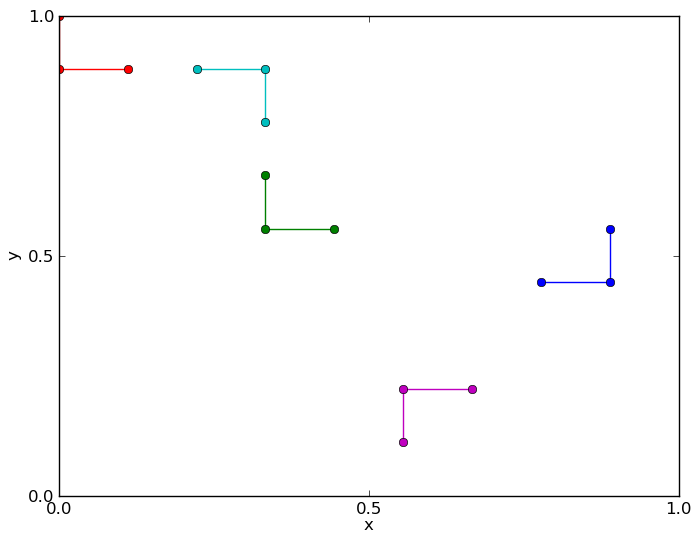
\includegraphics[width=0.50\textwidth]{./morris_alg.png}

\end{frame}
%%%%%%%%%%%%%%%%%%%%%%%%%%%%%%%%%%%%%%%%%%%%%%%%%%%%%%%%%%%%%%%%%%%%%%%%%%%%%%%%%%%%%%%%
\begin{frame}
\frametitle{Designing a Kriging Sampling Plan}

\begin{itemize}
  \item All surrogate models are built around a set of points at which the objective computer code is actually evaluated. 
  \item Intuitively, the surrogate accuracy is expected to decrease as one moves further away from such points. 
  \item Important to spread $N$ points as uniformly as possible across the design space.
  \item For Kriging, Latin Hypercube Sampling (LHS) is used to create a sampling plan.
  \item There is a notion of an optimized LHS sampling plan based on the maximin metric.   
\end{itemize}

\end{frame}
%%%%%%%%%%%%%%%%%%%%%%%%%%%%%%%%%%%%%%%%%%%%%%%%%%%%%%%%%%%%%%%%%%%%%%%%%%%%%%%%%%%%%%%%
\begin{frame}
\frametitle{Latin Hypercube Sampling}

\begin{itemize}
  \item Basis of LHS rests upon dividing the normalized space of each design variable into $n$ equally sized bins if $n$ samples are required. 
  \item As a result, when the $n$ samples are taken it is guaranteed that the entire
spectrum of each design variable's space has been visited.  
\end{itemize}
\centering
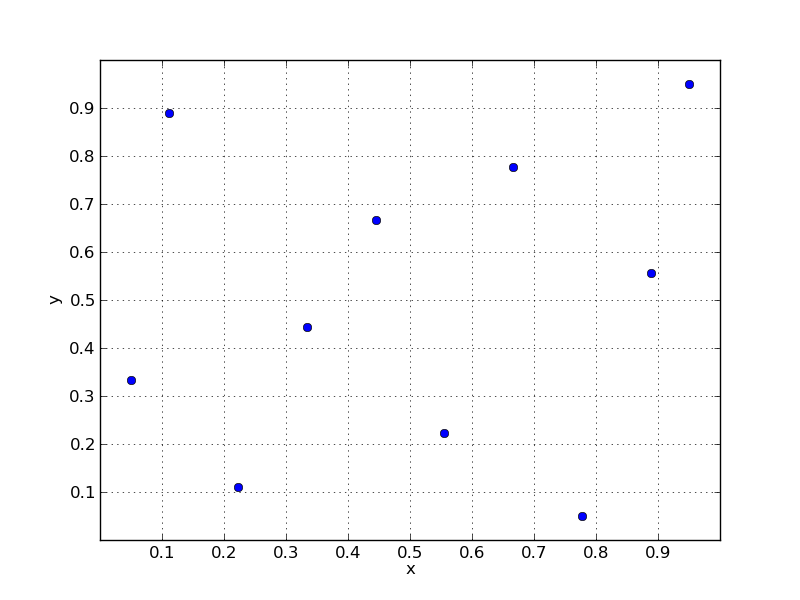
\includegraphics[width=0.58\textwidth]{./lhs.png}

\end{frame}
%%%%%%%%%%%%%%%%%%%%%%%%%%%%%%%%%%%%%%%%%%%%%%%%%%%%%%%%%%%%%%%%%%%%%%%%%%%%%%%%%%%%%%%%
\begin{frame}
\frametitle{Optimizing a LHS Plan}

\begin{itemize}
  \item The maximin metric describe by Morris and Mitchell makes use of two notions in an attempt to quantify the 'space-fillingness' of a sampling plan. 
  \item Unique distances between all points in the plan sorted in ascending order $\lbrace d_1, d_2, ..., d_m\rbrace$.
  \item Corresponding number of occurrences of each distance $\lbrace J_1, J_2, ..., J_m\rbrace$.  
  \item In words, the Morris and Mitchell criteria states that an optimized sampling plan will minimize all $J_i$ while maximizing the corresponding $d_i$. 
  \item The maximin sampling plan maximizes $d_1$, and among plans for which this is true, minimizes $J_1$, among plans for which this is true, maximizes $d_2$,....
\end{itemize}

\end{frame}
%%%%%%%%%%%%%%%%%%%%%%%%%%%%%%%%%%%%%%%%%%%%%%%%%%%%%%%%%%%%%%%%%%%%%%%%%%%%%%%%%%%%%%%%
\begin{frame}
\frametitle{Optimizing a LHS Plan}

\begin{itemize}
  \item The previous definition can be restated into a pseudo equivalent minimization problem.
\begin{equation}
\label{eq:Phi_q}
   \Phi_q(\textbf{X}) = \left(\sum_{j=1}^m J_j d_j^{-q} \right)^{1/q} \nonumber
\end{equation}
  \item The minimization of this equation and the Morris and Mitchell definition of the maximin sampling plan are used in unison to obtain a locally optimal sampling plan.
  \item Generate initial sampling plan, optimize for set of $q$ values using simulated annealing.  
  \item Resulting set of plans are contested directly against each other by explicit application of Morris and Mitchell's maximin definition. 
\end{itemize}

\end{frame}
%%%%%%%%%%%%%%%%%%%%%%%%%%%%%%%%%%%%%%%%%%%%%%%%%%%%%%%%%%%%%%%%%%%%%%%%%%%%%%%%%%%%%%%%
\begin{frame}
\frametitle{Kriging}

\begin{itemize}
  \item Linear regression is most commonly used surrogate to model a stochastic process.

\begin{equation}
   y\left( \textbf{x}^{(i)} \right) = \sum_h \beta_h f_h\left( \textbf{x}^{(i)} \right) + \epsilon^{(i)} \nonumber
\end{equation}

  \item The $\epsilon^{(i)}$ are normally distributed, independent error terms with mean $0$ and variance $\sigma^2$.
  \item The assumption of independent error terms is wrong. Errors are correlated. 
\end{itemize}

\end{frame}
%%%%%%%%%%%%%%%%%%%%%%%%%%%%%%%%%%%%%%%%%%%%%%%%%%%%%%%%%%%%%%%%%%%%%%%%%%%%%%%%%%%%%%%%
\begin{frame}
\frametitle{Kriging}

\begin{itemize}
  \item Given that error terms should be correlated, what if we modeled the error terms instead of the mean?

\begin{equation}
   d\left( \textbf{x}^{(i)}, \textbf{x}^{(j)} \right) = \sum_{h=1}^{k} \theta_h \left| x_h^{(i)} - x_h^{(j)} \right|^{p_h} \nonumber
\end{equation}

\begin{equation}
   \text{cor} \left[ \epsilon\left( \textbf{x}^{(i)} \right) , \epsilon\left( \textbf{x}^{(j)} \right)  \right] =
      \exp\left[ -d\left( \textbf{x}^{(i)}, \textbf{x}^{(j)} \right) \right]  \nonumber
\end{equation}

  \item This is what Kriging does.

\begin{equation}
   y\left( \textbf{x}^{(i)} \right) = \mu + \epsilon\left( \textbf{x}^{(i)} \right) \nonumber
\end{equation}

\end{itemize}

\end{frame}
%%%%%%%%%%%%%%%%%%%%%%%%%%%%%%%%%%%%%%%%%%%%%%%%%%%%%%%%%%%%%%%%%%%%%%%%%%%%%%%%%%%%%%%%
\begin{frame}
\frametitle{Kriging on a Sampling Plan}

\begin{itemize}
  \item Optimized sampling plan $\textbf{X}=\lbrace \textbf{x}^{(1)}, \textbf{x}^{(2)}, ... \textbf{x}^{(n)}\rbrace$. 
  \item At each datum $\textbf{x}^{(k)}$ a random process $Y(\textbf{x}^{(i)})$ induces an observation $y^{(i)}$.
  \item Resulting random field can be described with a mean value of $\textbf{1}\mu$ and a correlation matrix,
\begin{equation}
 \boldsymbol{\Psi} =
 \begin{pmatrix} 
	\text{cor} \left[ \epsilon\left( \textbf{x}^{(1)} \right) , \epsilon\left( \textbf{x}^{(1)} \right)  \right] & \cdots & 
		\text{cor} \left[ \epsilon\left( \textbf{x}^{(1)} \right) , \epsilon\left( \textbf{x}^{(n)} \right)  \right]  \\
	\vdots & \ddots & \vdots \\ 
	\text{cor} \left[ \epsilon\left( \textbf{x}^{(n)} \right) , \epsilon\left( \textbf{x}^{(1)} \right)  \right]  & \cdots & 
		\text{cor} \left[ \epsilon\left( \textbf{x}^{(n)} \right) , \epsilon\left( \textbf{x}^{(n)} \right)  \right] 
 \end{pmatrix} \nonumber
\end{equation}  

\end{itemize}

\end{frame}
%%%%%%%%%%%%%%%%%%%%%%%%%%%%%%%%%%%%%%%%%%%%%%%%%%%%%%%%%%%%%%%%%%%%%%%%%%%%%%%%%%%%%%%%
\begin{frame}
\frametitle{Kriging on a Sampling Plan}

\begin{itemize}
  \item Given the formulation of the observations occurring at $\textbf{x}^{(k)}$ as instances of a stochastic process, the likelihood of seeing the observed data is,
\begin{eqnarray}
   L\left(\textbf{Y}^{(1)}, ..., \textbf{Y}^{(n)} | 
    \mu, \sigma, \lbrace \theta_1,..., \theta_k\rbrace, 
    \lbrace p_1,..., p_k\rbrace\right) = \nonumber \\
     \frac{1}{\left(2\pi\sigma^2\right)^{n/2}|\boldsymbol{\Psi}|^{1/2}}\times
     \exp\left[\frac{  \left(\textbf{y}-\textbf{1}\mu\right)^T
    \boldsymbol{\Psi}^{-1} \left(\textbf{y}-\textbf{1}\mu\right)}
    {2\sigma^2} \right] . \nonumber
\end{eqnarray} 
  \item Maximizing the log likelihood, 
   \begin{equation}
   	\hat{\mu} = \frac{ \textbf{1}^T\boldsymbol{\Psi}^{-1}\textbf{y} }
    		 	    {  \textbf{1}^T\boldsymbol{\Psi}^{-1}\textbf{1} } \nonumber
   \end{equation}
   \begin{equation}
   	\hat{\sigma}^2 = \frac{  \left(\textbf{y}-\textbf{1}\mu\right)^T
    			\boldsymbol{\Psi}^{-1} \left(\textbf{y}-\textbf{1}\mu\right)}{n}. \nonumber
   \end{equation}
\end{itemize}

\end{frame}
%%%%%%%%%%%%%%%%%%%%%%%%%%%%%%%%%%%%%%%%%%%%%%%%%%%%%%%%%%%%%%%%%%%%%%%%%%%%%%%%%%%%%%%%
\begin{frame}
\frametitle{Kriging on a Sampling Plan}

\begin{itemize}
  \item Substitute $\hat{\sigma}$ and $\hat{\mu}$ into log likelihood to get, concentrated ln-likelihood function.
   \begin{equation}
    \log(L) \approx -\frac{n}{2}\log\left(\hat{\sigma}^2\right) -
     \frac{1}{2} \log|\boldsymbol{\Psi}| \nonumber	
   \end{equation}
  \item Optimize with respect to the $\theta$ and $p$ parameters using global search algorithm.
  \item Once all optimizing parameters are available the goal is to utilize the parameters to build a model that makes function predictions on new points $\textbf{x}$.
\end{itemize}

\end{frame}
%%%%%%%%%%%%%%%%%%%%%%%%%%%%%%%%%%%%%%%%%%%%%%%%%%%%%%%%%%%%%%%%%%%%%%%%%%%%%%%%%%%%%%%%
\begin{frame}
\frametitle{Making Predictions with Kriging Surrogate}

\begin{itemize}
  \item Construct a vector of correlations with existing points and $\textbf{x}$,
   \begin{equation}
 	\boldsymbol{\psi} =
 	\begin{pmatrix} 
	 \text{cor} \left[ \epsilon\left( \textbf{x}^{(1)} \right) , \epsilon\left( \textbf{x} \right)  \right]  \\
	 \vdots \\ 
	 \text{cor} \left[ \epsilon\left( \textbf{x}^{(n)} \right) , \epsilon\left( \textbf{x} \right)  \right] 
    \end{pmatrix}. \nonumber
   \end{equation} 
  \item  New predictions can be made at $\textbf{x}$ using the maximum likelihood estimator,
   \begin{equation}
    \hat{y}(\textbf{x}) = \hat{\mu} + 
   	 \boldsymbol{\psi}^T\boldsymbol{\Psi}^{-1}
   	  \left(\textbf{y} - \textbf{1}\hat{\mu}\right). \nonumber
   \end{equation}
  \item Prediction using kriging works to estimate a function value at a certain point by computing a weighted average of known function values in the vicinity of the objective points.
\end{itemize}

\end{frame}